\chapter{Konvergente Reihen}
%Chapter: 5
\begin{fsatz}[Endliche geometrische Reihe]
F�r alle $q \in \mb{R} \backslash \gklamm{1}$ und $n \in \mb{N}_0$ gilt:
\[\sum_{k = 0}^n q^k = \frac{1 - q^{n +1}}{1 - q}\]
\end{fsatz}

\begin{fbeweis}[Vollst�ndige Induktion]
\mbox{}\par
\begin{description}
\item[(IA)] $n = 0$
		\[\left.\begin{array}{l}\tx{LS } = \sum_{k = 0}^0 q^k = q^0 = 1\\\tx{RS } = \frac{1 - q^1}{1 - q} = 1\end{array}\right\} \checkmark\]
\item[(IS)] \ac{z.z.} $\forall n \in \N_0: \underbrace{\rkl{\sum_{k = 0}^n = q^k = \frac{1 - q^{n + 1}}{1 - q}}}_{\tx{(IV)}} \Ra \sum_{k = 0}^{n + 1} q^k = \frac{1 - q^{n + 2}}{1 - q}$
\begin{align*}
&\sum_{k = 0}^{n + 1} q^k = q^{n + 1} + \sum_{k = 0}^n q^k \stack{=}{\tx{(IV)}} q^{n + 1} + \frac{1 - q^{n + 2}}{1 - q}\\
= & \frac{q^{n + 1} - q^{n + 2} + 1 - q^{n + 1}}{1 - q} = \frac{1 - q^{n + 2}}{1 - q}
\end{align*}
\end{description}\qed
\end{fbeweis}

\begin{fdefinition}[Unendliche Reihen]
%MARK: Definition 2.9
Sei die Folge $(A_k)_{k \in \mb{N}}$ gegeben. Die Folge $(S_n)_{n \in \mb{N}}$ der \indexb{Partialsummen} ist definiert durch
\[S_n \ceq \sum_{k = 1}^n A_k\]
Man nennt $(S_n)_{n \in \mb{N}}$ auch \indexb{unendliche Reihe} mit den Gliedern $A_k$ (geschrieben $\sum_{k = 1}^{\infty} A_k$ oder $\sum A_k$).\\
Wenn die Folge $(S_n)_{n \in \mb{N}}$ konvergiert, nennt man auch die Reihe $\sum_{k = 1}^{\infty} A_k$ konvergent und $S \ceq \lim_{n \ra \infty} S_n = \sum_{k = 1}^{\infty} A_k$ ist der Wert der Summe.
\end{fdefinition}

\begin{bemerkung}
Unendliche Reihen k�nnen bei einem beliebigen Index $k \in \mb{Z}$ beginnen ($\sum_{k = j}^{\infty} A_k$) meistens $j = 0$ oder $j = 1$.
\end{bemerkung}

\begin{fsatz}[Unendliche geometrische Reihe]
F�r die (unendliche) geometrische Reihe gilt:
\[\sum_{k = 0}^{\infty} q^k \text{ ist divergent f�r } \betrag{q} \grgl 1\]
\[S \ceq \sum_{k = 0}^{\infty} q^k = \frac{1}{1 - q} \tx{ f�r } \betrag{q} < 1\]
\end{fsatz}

\begin{fbeweis}
\mbox{}\par
\begin{description}
\item[Fall 1] $\betrag{q} < 1$
		\[S = \lim_{n \ra \infty} S_n = \lim_{n \ra \infty} \sum_{k = 0}^n = A_k \underbrace{=}_{\text{Satz 2.8}} \lim_{n \ra \infty} \frac{1 - q^{n + 1}}{1 - q} = \frac{1}{1 - q}\]
\item[Fall 2] $\betrag{q} > 1$
		\[S_n = \sum_{k = 0}^n A_k = \frac{1 - q^{n + 1}}{1 - q}\]
		ist nicht beschr�nkt, da $q^{n + 1}$ f�r $\betrag{q} > 1$ divergent
		\begin{itemize}[label=\Ra]
		\item $(S_n)_{n \in \mb{N}}$ divergent
		\item $\sum_{k = 0}^{\infty} A_k$ divergent
		\end{itemize}

\item[Fall 3] $q = 1$
		\[ S_n = \sum_{k = 0}^n 1^k = n + 1 \stack{n \ra \infty}{\longrightarrow} \infty\]
		\begin{itemize}[label=\Ra]
		\item $(S_n)_{n \in \mb{N}}$ divergent
		\item $\sum_{k = 0}^{\infty} A_k$ divergent
		\end{itemize}

\item[Fall 4] $q = -1$
		\[S_n = \sum_{k = 0}^n (-1)^k = \begin{cases}1 \text{ f�r } n \tx{ gerade}\\0 \tx{ f�r } n \tx{ ungerade}\end{cases}\]
		\begin{itemize}[label=\Ra]
		\item $(S_n)_{n \in \mb{N}}$ divergent
		\item $\sum_{k = 0}^{\infty} A_k$ divergent
		\end{itemize}
\end{description}\qed
\end{fbeweis}

\begin{fsatz}[Konvergenzkriterien f�r Reihen]
\mbox{}\par
\begin{enumerate}[label=\roman*)]
\item Notwendiges Kriterium\\
		\[\sum_{k = 0}^{\infty} A_k \tx{ konvergent } \Ra \lim_{k \to \infty} A_k = 0\]
		Dies ist aber kein zwingendes Kriterium f�r Konvergenz eher f�r das Beweisen der Divergenz geeignet.

\item Leibnitz-Kriterium (f�r alternierende Reihen)\\
		Wenn $(A_k)_{k \in \N}$ eine monoton fallende Nullfolge ist, dann konvergiert die alternierende Reihe
		\[\sum_{k = 1}^{\infty} (-1)^k \mal A_k\]

\item Vergleichskriterien\\
		Sei $\betrag{A_k} \klgl B_k \forall k \grgl k_0$ dann gilt:
		\begin{enumerate}[label=\alph*)]
		\item Majorantenkriterium\\
				$\sum_{k = 0}^{\infty} B_k$ konvergent
				\begin{itemize}[label=\Ra]
				\item $\sum_{k = 0}^{\infty} \betrag{A_k}$ konvergent
				\item $\sum_{k = 0}^{\infty} A_k$ konvergent
				\end{itemize}

		\item Minorantenkriterium\\
				$\sum_{k = 0}^{\infty} \betrag{A_k}$ divergent
				\begin{itemize}[label=\Ra]
				\item $\sum_{k = 0}^{\infty} B_k$ divergent
				\end{itemize}
		\end{enumerate}

\item Wurzelkriterium
		\[\lim_{k \ra \infty} \sqrt[k]{\betrag{A_k}} = w = \begin{cases}< 1 & \Ra \sum_{k = 0}^{\infty} A_k, \sum_{k = 0}^{\infty} \betrag{A_k} \tx{ konvergent}\\> 1 & \Ra \sum_{k = 0}^{\infty} A_k, \sum_{k = 0}^{\infty} \betrag{A_k} \tx{ divergent}\end{cases}\]

\item Quotientenkriterium
		\[\lim_{k \ra \infty} \betrag{\frac{A_{k + 1}}{A_k}} = q = \begin{cases}< 1 & \Ra \sum_{k = 0}^{\infty} A_k, \sum_{k = 0}^{\infty} \betrag{A_k} \tx{ konvergent}\\> 1 & \Ra \sum_{k = 0}^{\infty} A_k, \sum_{k = 0}^{\infty} \betrag{A_k} \tx{ divergent}\end{cases}\]
\end{enumerate}
\end{fsatz}

\begin{fbeweis}
\mbox{}\par
\begin{enumerate}[label=\roman*)]
\item Kontraposition \ac{z.z.}
		\[\neg \rkl{\lim_{k \ra \infty} A_k = 0} \Ra \sum A_k \tx{ divergent}\]
		$A_k$ keine Nullfolge
		\begin{align*}
		&\exists \epsilon > 0~\forall N(\epsilon)~\exists n \grgl N(\epsilon):~\betrag{A_k - 0} > \epsilon\\
		\Lra &\exists \epsilon > 0 ~ \forall \N_0 \in \N ~ \exists n \grgl \N_0:~\betrag{A_n} > \epsilon\\
		&\betrag{S_n - S_{n - 1}} = \betrag{A_n} > \epsilon\\
		&\Ra \forall S \in \mb{R}:~\max \rkl{\betrag{S - S_n}, \betrag{S - S_{n - 1}}} > \frac{\epsilon}{2}
		\end{align*}

		%MA-02.04.2009-IMG-2
		\begin{tikzpicture}[decoration=brace]
		\foreach \x in {0, 0.5, 1,..., 5}
			\draw (\x,0) rectangle +(0.3,0.2);
		
		\draw[decorate] (5.3,-0.2) -- (3.5,-0.2) node[below,midway] {m�gl. Positionen};
		\draw[decorate] (4.8,-1) -- (1.5,-1) node[below,midway] {m�gl. Positionen};
		\end{tikzpicture}

\item $A_{k + 1} \klgl A_k$ $S_n = \sum_{k = 1}^n (- 1)^k A_k$

		%MA-07.04.2009-IMG-1
		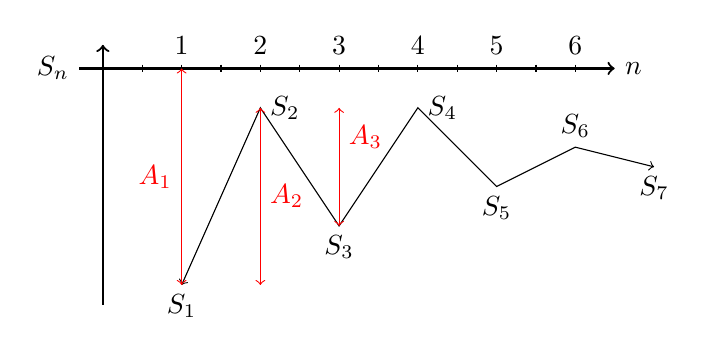
\begin{tikzpicture}
		\draw[->, thick] (-0.3,0) node[left] {$S_n$} -- (6.5,0) node[right] {$n$};
		\draw[<-, thick] (0,0.3) -- (0,-3);
		
		\foreach \x in {0.5, 1.5,...,5.5}
			\draw (\x,0.05) -- (\x,-0.05);
		
		\foreach \x in {1, 2,...,6}
			\draw (\x,0.05) node[above] {$\x$} -- (\x,-0.05);
		
		\draw[<->] (1,-2.75) node[below] {$S_1$} -- (2,-0.5) node[right] {$S_2$} -- (3,-2) node[below] {$S_3$} -- (4,-0.5) node[right] {$S_4$} -- (5,-1.5) node[below] {$S_5$} -- (6,-1) node[above] {$S_6$} -- (7,-1.25) node[below] {$S_7$};
		
		\draw[<->, draw=red] (1,0) -- (1,-2.75) node[left,midway,color=red] {$A_1$};
		\draw[<->, draw=red] (2,-0.5) -- (2,-2.75) node[right,midway,color=red] {$A_2$};
		\draw[<->, draw=red] (3,-0.5) -- (3,-2) node[right,near start,color=red] {$A_3$};
		\end{tikzpicture}

		\[\underbrace{S_1 \klgl S_3 \klgl S_5 \klgl \dots \klgl S_{2n + 1}}_{\begin{minipage}{35mm}\begin{center}\scriptsize{monoton wachsende $n$ nach oben beschr�nkt Folge mit $T \ceq \lim_{n \ra \infty} s_{2n + 1}$}\end{center}\end{minipage}} \klgl S \klgl \underbrace{S_{2n} \klgl \dots \klgl S_6 \klgl S_4 \klgl S_2}_{\begin{minipage}{32mm}\begin{center}\scriptsize{monoton fallende und nach unten beschr�nkte Folge mit $U \ceq \lim_{n \ra \infty} s_{2n}$}\end{center}\end{minipage}}\]
		\begin{align*}
		U - T &= \lim_{n \ra \infty} \rklamm{S_{2n}} - \lim_{n \ra \infty} \rklamm{S_{2 n + 1}} = \lim_{n \ra \infty} \rklamm{S_{2n} - S_{2n + 1}}\\
		&= \lim_{n \ra \infty} \rklamm{\sum_{k = 1}^{2n} (-1)^k A_k - \sum_{k = 1}^{2n + 1} (-1)^k A_k}\\
		&= \lim_{n \ra \infty} -(-1)^{2n + 1} \mal A_{2n + 1} = \lim_{n \ra \infty} A_{2n + 1} = 0\\
		&\Ra \lim_{n \ra \infty} S_n = S(= T = U)
		\end{align*}

\item \begin{enumerate}[label=\alph*)]
		\item Majorantenkriterium
				\begin{itemize}
				\item es gilt $\sum_{k = 0}^{\infty} B_k$ konvergent und $\forall k \grgl k_0$ $0 \klgl \betrag{A_k} \klgl B_k$
				\item $\sum B_k$ konvergent
						\begin{align*}
						\Lra &\forall \epsilon > 0 \exists N(\epsilon) \forall n \grgl N(\epsilon)\\
						&\betrag{\underbrace{\sum_{k = 0}^n B_k - \sum_{k = 0}^{\infty}}_{\sum_{k = n + 1}^{\infty} B_k}} < \epsilon
						\end{align*}
						$n \grgl \max(N, k_0)$
						\[\betrag{\sum_{k = 0}^n A_k - \sum_{k = 0}^{\infty} A_k} = \betrag{\sum_{k = n + 1}^{\infty} A_k} \klgl \sum_{k = n + 1}^{\infty} \betrag{A_k} \klgl \sum_{k = n + 1}^{\infty} B_k \klgl \epsilon\]
						\Ra $\sum_{k = 0}^{\infty} \betrag{A_k}$ konvergent; $\sum_{k = 0}^{\infty} A_k$ konvergent\\
						Nebenergebnis:
						$\sum \betrag{A_k}$ konvergent \Ra $\sum A_k$ konvergent
				\end{itemize}
		\item Minorantenkriterium\\
%				$\sum \betrag{A_k} \tx{ divergent}}_{\Lra \sum \betrag{A_k} = \infty}$ und $\forall k \grgl k_0 \mal \betrag{A_k} \klgl B_k$
				\[\sum_{k = 0}^{\infty} B_k = \sum_{k = k_0}^{\infty} B_k \grgl \sum_{k = k_0}^{\infty} \betrag{A_k} = \infty\]
				\Ra $\sum_{k = 0}^{\infty} B_k$ divergent
		\end{enumerate}

\item Wurzelkriterium
		\begin{description}
		\item[Fall 1] $w < 1$
				\begin{align*}
				\lim_{k \ra \infty} \sqrt[k]{\betrag{A_k}} = w < 1 \Lra &\forall \epsilon > 0 \exists N(\epsilon) \forall n \grgl N (\epsilon)\\
				&\betrag{\sqrt[n]{\betrag{a_n}} - w} < \epsilon
				\end{align*}
				\begin{align*}
				\Ra &\sqrt[n]{\betrag{A_n}} - w < \epsilon\\
				\Lra &\sqrt[n]{\betrag{A_n}} < \epsilon + w = q\\
				\Ra & \betrag{A_n} < q^n\\
				&\tx{Sei $\epsilon$ so klein, dass $q < 1$}
				\end{align*}
				\begin{align*}
				\Ra 0 &\klgl \sum_{k = 0}^{\infty} \betrag{A_k} = \sum_{k = 0}^{N - 1} \betrag{A_k} + \sum_{k = N}^{\infty} \betrag{A_k} \klgl \sum_{k = 0}^{N - 1} \betrag{A_k} + \sum_{k = N}^{\infty} q^k\\
				&\klgl \underbrace{\sum_{k = 0}^{N - 1} \betrag{A_k}}_{\begin{minipage}{18mm}\begin{center}\scriptsize{End Summe \Ra konvergent}\end{center}\end{minipage}} + \underbrace{\sum_{k = 0}^{\infty} q^n}_{\begin{minipage}{18mm}\begin{center}\scriptsize{konvergent (geometrische Reihe mit $q < 1$)}\end{center}\end{minipage}} < \infty
				\end{align*}
				\Ra $\sum \betrag{A_k}$ konvergent \Ra $\sum A_k$ konvergent

		\item[Fall 2] $w > 1$
				\begin{align*}
				\lim_{k \ra \infty} \sqrt[k]{\betrag{A_k}} = w > 1 \Lra &\forall \epsilon > 0 \exists N(\epsilon): \forall n \grgl N(\epsilon)
				&\betrag{\sqrt[q]{\betrag{A_n}} - w} < \epsilon
				\end{align*}
				\begin{align*}
				\Ra & - \epsilon < \sqrt[n]{\betrag{A_n}} - w\\
				\Lra & \underbrace{w - \epsilon}_{= Q} < \sqrt[n]{\betrag{A_n}}\\
				\Ra & Q^n < \betrag{A_n}\\
				&\tx{$\epsilon$ so klein, dass $Q = w - \epsilon > 1$}
				\end{align*}
				\[\sum_{k = 0}^{\infty} \betrag{A_k} = \sum_{k = N - 1}^{\infty} \betrag{A_k} + \sum_{k = N}^{\infty} \betrag{A_k} \grgl \sum_{k = N}^{\infty} \betrag{A_k} \grgl \sum_{k = N}^{\infty} Q^k = \infty\]
				\Ra $\sum \betrag{A_k}$ divergent (Rechnung f�r $\sum_{A_k}$ analog)
		\end{description}

\item Beweis Quotientenkriterium �hnlich wie Wurzelkriterium \qed
\end{enumerate}
\end{fbeweis}

\begin{fsatz}[Cauchyscher Verdichtungssatz]
Sei $(A_k)_{k \in \N}$ monoton fallend ($A_K > 0$), dann gilt
\[\sum_{k = 1}^{\infty} \tx{ konvergent } \Lra \sum_{k = 0}^{\infty} 2^k \mal A_{2k} \tx{ konvergent}\]
\end{fsatz}

\begin{fbeweis}
Zu zeigen $\sum_{k = 1}^{2^{n + 1} - 1} A_k \klgl \sum_{k = 0}^n 2^k A_{2k} \klgl 2 \sum_{k = 1}^{2n} A_k$
\end{fbeweis}

\begin{beispiel}
\mbox{}\par
\begin{enumerate}
\item Harmonische Reihe: $\sum_{k = 1}^{\infty} \underbrace{\frac{1}{k}}_{A_k}$ divergent, denn $\sum 2^k \mal \frac{1}{2^k} = \sum_{k = 1}^{\infty} 1 = \infty$ \Ra $\sum 2^k \mal \frac{1}{2^k}$ divergent. Damit ist nach dem Verdichtungssatz auch $\sum_{k = 1}^{\infty} \frac{1}{k}$ divergent
\item Alternierende harmonische Reihe
		\[\sum_{k = 1}^{\infty} (-1)^k \mal \frac{1}{k} = \mathbf{- \ln(2)}\]
		konvergent nach Leibnitz, da $A_k \frac{1}{k}$ monoton fallend mit $\lim_{k \ra \infty} A_k = \lim_{k \ra \infty} \frac{1}{k} = 0$

\item Verallgemeinerte harmonische Reihe
		\[\sum_{k = 1}^{\infty} \frac{1}{k^{\alpha}} = \begin{cases}\alpha > 1 & \tx{konvergent}\\\alpha \klgl 1 & \tx{divergent}\end{cases}\]
		Wir betrachten
		\[\sum_{k = 0}^{\infty} 2^k \mal \frac{1}{\rklamm{2^k}^{\alpha}} = \sum_{k = 0}^{\infty} 2^{k (1 - \alpha)} = \sum_{k = 0}^{\infty} \rklamm{2^{1 - \alpha}}^k\]
		\begin{itemize}
		\item divergent f�r $\alpha \klgl 1$ (da $^{1 - \alpha} \grgl 1$ und geometrische Reihe daf�r divergent)
		\item konvergent f�r $\alpha > 1$ (da $2^{1 - \alpha} < 1$ und geometrische Reihe f�r $q < 1$ konvergent)
		\end{itemize}
		\[\sum_{k = 1}^{\infty} \frac{1}{k^2} = \frac{\pi^2}{6}\]

\item $\sum_{k = 0}^{\infty} \frac{x^k}{k!}$, $x \in \mb{R}$\\
		Quotientenkriterium
		\begin{align*}
		&\lim_{k \ra \infty} \betrag{\frac{A_{k + 1}}{A_k}} = \lim_{k \ra \infty} \betrag{\frac{x^{k + 1}}{(k + 1)!} \mal \frac{k!}{x^k}}
		=& \lim_{k \ra \infty} \betrag{\frac{x}{k + 1}} = \betrag{x} \mal \lim_{k \ra \infty} \frac{1}{k + 1} = 0 < 1
		\end{align*}
		\Ra $\sum_{k = 0}^{\infty} \frac{x^k}{k!}$
\end{enumerate}
\end{beispiel}

\section{Aufgabe 2.3}
\label{sec:Konvergente_Reihen_A2_3}
Untersuchen Sie die folgenden Reihen auf Konvergenz:
\begin{enumerate}[label=\alph*)]
\item $\sum_{n = 1}^{\infty} \frac{1}{2+ 3^n}$
\item $\sum_{n = 1}^{\infty} \sqrt[n]{n^2}$
\item $\sum_{k = 1}^{\infty} (-1)^{k + 1} \frac{k^2}{k^3 + 1}$
\end{enumerate}

L�sung siehe \vref{sec:Konvergente_Reihen_A2_3L}.

\section{Aufgabe 2.4}
\label{sec:Konvergente_Reihen_A2_4}
F�r welche Werte von $r$ konvergiert die Reihe
\[1+2r+r^2+2r^3+r^4+2r^5+r^6+\dots\]
Bestimmen Sie im Fall der Konvergenz den Grenzwert.

L�sung siehe \vref{sec:Konvergente_Reihen_A2_4L}.

\begin{fsatz}[Cauchy-Produkt]
%MARK: Satz 2.13
Seien $\sum_{k = 0}^{\infty} \betrag{A_k}$ und $\sum_{k = 0}^{\infty} \betrag{B_k}$ konvergente Reihen. Dann ist
\[\rklamm{\sum_{k = 0}^{\infty} A_k} \mal \rklamm{\sum_{k = 0}^{\infty} B_k} = \sum_{k = 0}^{\infty} C_k\]
mit $C_k = \sum_{l = 0}^{k} A_l \mal B_{k - l}$
\end{fsatz}

\begin{beweis}
-
\end{beweis}

\section{L�sungen}
\subsection{Aufgabe 2.3}
\label{sec:Konvergente_Reihen_A2_3L}
L�sung zu Aufgabe \vref{sec:Konvergente_Reihen_A2_3}.

\begin{enumerate}[label=\alph*)]
\item $\sum_{n = 1}^{\infty} \frac{1}{2+ 3^n}$
		\begin{itemize}
		\item notwendiges Kriterium
				\[\lim_{n \ra \infty} A_n = \lim_{n \ra \infty} \frac{1}{2 + 3^n} = 0 \Ra \sum A_n \tx{ kann konvergent sein}\]

		\item Majorantenkriterium
				\[\sum_{n = 1}^{\infty} \frac{1}{2 + 3^n} \klgl \ubl{\sum_{n = 1}^{\infty} \rklamm{\frac{1}{3}}^n}{konvergente geometrische Reihe} \Ra \tx{ konvergent}\]

		\item Quotientenkriterium
				\begin{align*}
				\lim_{n \ra \infty} \betrag{\frac{A_{n + 1}}{A_n}} &= \lim_{n \ra \infty} \betrag{\frac{1}{2 + 3^{n + 1}} \mal \frac{2 + 3^n}{1}} = \lim_{n \ra \infty} \frac{2 + 3^n}{2 + 3^{n + 1}}\\
				&= \lim_{n \ra \infty} \frac{\frac{2}{3^n} + 1}{\frac{2}{3^n} + 3} = \frac{\lim_{n \ra \infty} \rklamm{\frac{2}{3^n} + 1}}{\lim_{n \ra \infty} \rklamm{\frac{2}{3^n} + 3}} = \frac{1}{3}\\
				&\Ra \tx{ konvergent}
				\end{align*}

		\item Wurzelkriterium
				\begin{align*}
				&0 \klgl \lim_{n \ra \infty} \sqrt[n]{\betrag{A_n}} = \lim_{n \ra \infty} \sqrt[n]{\betrag{\frac{1}{2 + 3^n}}} \klgl \lim_{n \ra \infty} \sqrt[n]{\frac{1}{3^n}} = \lim_{n \ra \infty} \frac{1}{3} = \frac{1}{3}\\&
				\Ra \tx{ konvergent}
				\end{align*}

		\item Verdichtungssatz
				\[\sum_{n = 0}^{\infty} 2^n \mal \frac{1}{\underbrace{2 + 3^{2^n}}_{= A_{2^n}}} \klgl \sum_{n = 0}^{\infty} 2^n \mal \rklamm{\frac{1}{3^2}}^n = \ubl{\sum_{n = 0}^{\infty} \rklamm{\frac{2}{9}}^n}{konvergente geometrische Reihe}\]
				\[\sum_{n = 0}^{\infty} 2^n \frac{2}{2 + 3^{2^n}} \tx{ konvergent } \Lra \sum_{n = 1}^{\infty} \frac{1}{2 + 3^n} \tx{ konvergent}\]
		\end{itemize}

\item $\sum_{n = 1}^{\infty} \sqrt[n]{n^2}$
		notwendiges Kriterium:
		\[\lim_{n \ra \infty} A_n = \lim_{n \ra \infty} \sqrt[n]{n^2} = \rklamm{\lim_{n \ra \infty} \sqrt[n]{n}}^2 = 1 \Ra \tx{ divergent}\]

\item $\sum_{k = 1}^{\infty} (-1)^{k + 1} \frac{k^2}{k^3 + 1}$
		\begin{description}
		\item[Leibnitz Kriterium] $A_K = \frac{k^2}{k^3 + 1}$
				\[\lim_{n \ra \infty} A_k = \lim_{k \ra \infty} \frac{k^2}{k^3 + 1} = \lim_{n \ra \infty} \frac{1}{k + \frac{1}{k^2}} = 0\]
				$(A_k)$ Nullfolge

		\item[Monoton fallend] zu zeigen $\frac{(k + 1)^2}{(k + 1)^3 + 1} < \frac{k^2}{k^3 + 1}$
				$\Ra \sum_{k = 1}^{\infty} (-1) \frac{k^2}{k^3 + 1}$ konvergent
		\end{description}
\end{enumerate}

\subsection{Aufgabe 2.4}
\label{sec:Konvergente_Reihen_A2_4L}
L�sung zu Aufgabe \vref{sec:Konvergente_Reihen_A2_4}.

$1+2r+r^2+2r^3+r^4+2r^5 + \dots$
\begin{align*}
&\sum_{k = 0}^{\infty} r^{2k} + 2 \sum_{k = 0}^{\infty} r^{2k + 1}\\
&= \sum_{k = 0}^{\infty} \rklamm{r^2}^k + 2r \sum_{k = 0}^{\infty} \rklamm{r^2}^k\\
\end{align*}
konvergent \Lra $r^2 < 1$ \Lra $r \in (-1, 1)$
